\textbf{See the instruction for questions \inteval{\value{question}+1} to \inteval{\value{question}+3}.}

\begin{center}
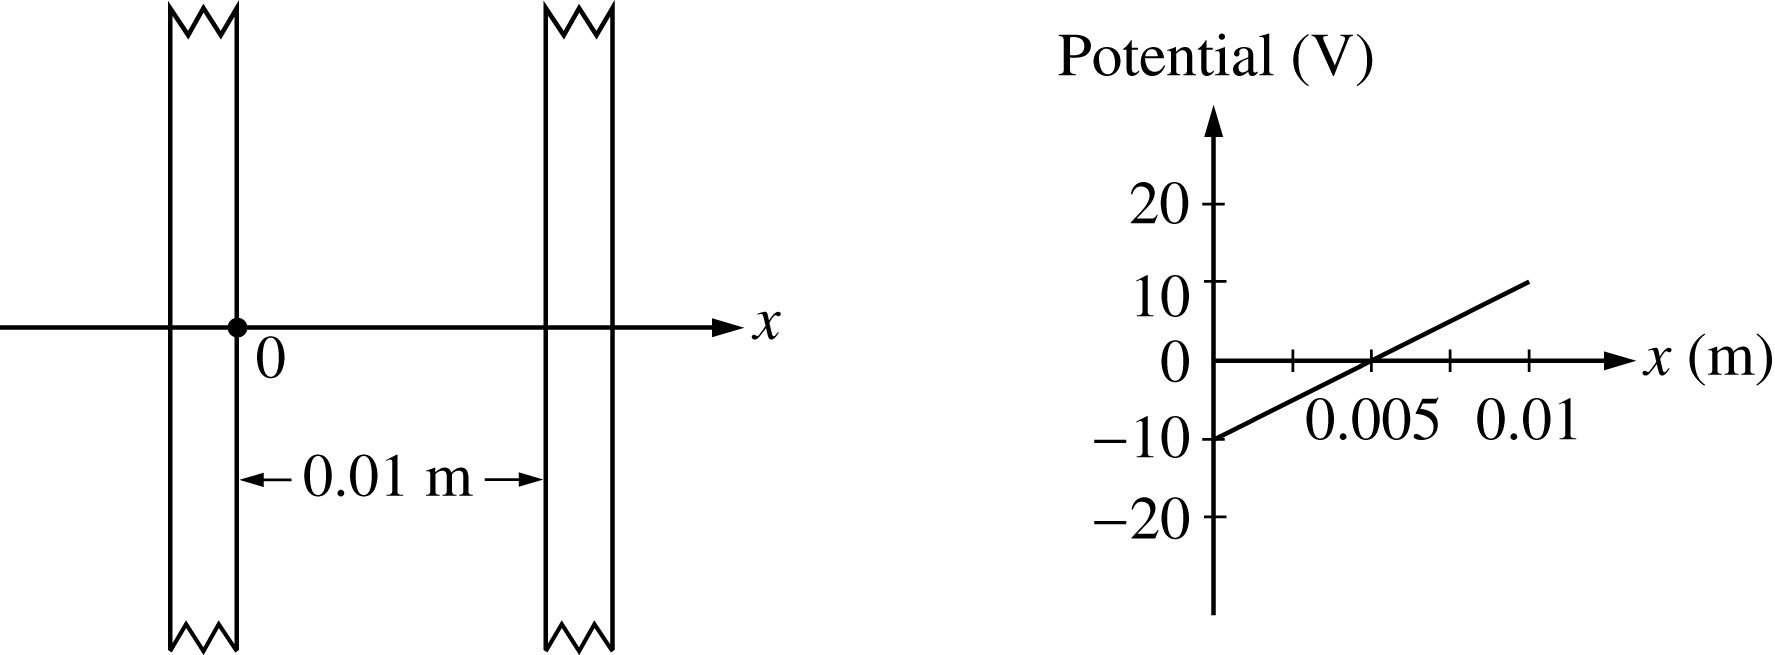
\includegraphics[scale=0.2]{images/img-003-002.png}
\end{center}

A uniform electric field exists between two parallel plates that are perpendicular to an $x$-axis and separated by $0.01 \unit{m}$, as shown above on the left. The graph above on the right shows the electric potential between the plates as a function of position $x$ on the $x$-axis.

% Multiple Choice Question 2
\begin{questions}\setcounter{question}{1}\question
What is the electric potential energy of an object with a $1.0 \unit{\mu C}$ charge located at $x=0.005 \unit{m}$ ?

\begin{oneparchoices}
\choice $-20 \unit{\mu J}$
\choice $-10 \unit{\mu J}$
\choice Zero
\choice $10 \unit{\mu J}$
\choice $20 \unit{\mu J}$
\end{oneparchoices}\end{questions}

% Multiple Choice Question 3
\begin{questions}\setcounter{question}{2}\question
What is the magnitude of the electric field between the plates at $x=0.005 \unit{m}$ ?

\begin{oneparchoices}
\choice Zero
\choice $0.1 \unit{V / m}$
\choice $0.2 \unit{V / m}$
\choice $1000 \unit{V / m}$
\choice $2000 \unit{V / m}$
\end{oneparchoices}\end{questions}

% Multiple Choice Question 4
\begin{questions}\setcounter{question}{3}\question
What is the direction of the electric field between the plates at points on the $x$-axis?

\begin{choices}
\choice To the left at all points
\choice To the right at all points
\choice To the left for $x<0.005 \unit{m}$ and to the right for $x>0.005 \unit{m}$
\choice To the right for $x<0.005 \unit{m}$ and to the left for $x>0.005 \unit{m}$
\choice It is undefined because the field is zero at all points.
\end{choices}\end{questions}

